\documentclass{article}
\usepackage[T1]{fontenc}
\usepackage{lmodern}
\usepackage[paperwidth=1189mm, paperheight=841mm, margin=40mm, top=35mm]{geometry}
\usepackage{xcolor}
\usepackage{multicol}
\usepackage{titlesec}
\usepackage{enumitem}
\usepackage{booktabs}
\usepackage{amsmath}
\usepackage{tikz}
\usepackage{pgfplots}
\pgfplotsset{compat=1.18}

% Colours used for headings, rules and highlights.
\definecolor{deep}{HTML}{264653}
\definecolor{sea}{HTML}{2A9D8F}
\definecolor{sand}{HTML}{E9C46A}
\definecolor{clay}{HTML}{E76F51}

% Text sizes for an A0 landscape poster.
\newcommand{\bodysize}{\fontsize{38}{50}\selectfont}
\newcommand{\smallsize}{\fontsize{29}{37}\selectfont}

\pagestyle{empty}
\setlength{\parindent}{0pt}
\setlength{\parskip}{16pt}
\setlength{\columnsep}{36mm}
\setlength{\columnseprule}{2pt}
\renewcommand{\columnseprulecolor}{\color{sea!40}}
\setlist{leftmargin=1.3em, itemsep=8pt, topsep=8pt}

% Numbered section headings with a coloured bar underneath.
\titleformat{\section}{\fontsize{56}{64}\selectfont\bfseries\sffamily\color{deep}}
  {\textcolor{clay}{\thesection}}{0.5em}{}[\vspace{-8pt}\textcolor{sea}{\rule{\linewidth}{5pt}}]
\titlespacing*{\section}{0pt}{40pt}{24pt}

% A shaded highlight box that fits inside a column.
\newcommand{\keypoint}[1]{\par\smallskip\colorbox{sand!35}{\parbox{\dimexpr\linewidth-2\fboxsep}{\vspace{12pt}\bfseries #1\vspace{12pt}}}\par}

\begin{document}
\bodysize

% Title block: edit the title, authors and affiliation.
\begin{minipage}[c]{0.78\linewidth}
  {\fontsize{110}{120}\selectfont\bfseries\sffamily\color{deep} Honeybee Foraging Under Heat Stress\par}
  \vspace{18mm}
  {\fontsize{46}{54}\selectfont\sffamily Rosa Delgado, Tomasz Wr\'oblewski and Aiko Tanaka\par}
  \vspace{8mm}
  {\fontsize{36}{44}\selectfont\sffamily\color{sea} Pollinator Ecology Group, Example Agricultural University\par}
\end{minipage}\hfill
\begin{minipage}[c]{0.18\linewidth}
  \raggedleft
  \tikz\node[draw=deep, line width=3pt, minimum width=170mm, minimum height=110mm, font=\smallsize]{Logo placeholder};
\end{minipage}

\vspace{20mm}
{\color{deep}\rule{\linewidth}{10pt}}
\vspace{10mm}

\begin{multicols}{3}

\section{Background}
Honeybees pollinate a third of the crops we eat. As summers get hotter, colonies may spend more energy cooling the hive and less on foraging.

We asked how daily maximum temperature changes the number of foraging trips and the pollen brought home.

\keypoint{Hypothesis: foraging trips fall steeply above 34\,\textdegree C.}

\section{Methods}
\begin{itemize}
  \item 18 colonies across three farms, June to August.
  \item Entrance counters logged every departure and return.
  \item Pollen traps emptied daily and weighed dry.
  \item Local weather stations recorded temperature.
\end{itemize}

We fitted a piecewise regression with an unknown breakpoint $\tau$:
\[ \text{trips} = \alpha + \beta_1 T + \beta_2 (T - \tau)_{+} \]

\centering
% Replace with a photo placeholder or your own drawing.
\tikz\node[draw=gray, line width=2pt, fill=gray!10, minimum width=0.95\linewidth, minimum height=110mm]{Image placeholder};
\par\smallsize Hive entrance counter used in the study.
\raggedright\bodysize

\columnbreak

\section{Results}
Trips rose gently with temperature until about 33\,\textdegree C, then dropped by a third.

\begin{center}
  % Edit these coordinates to plot your data.
  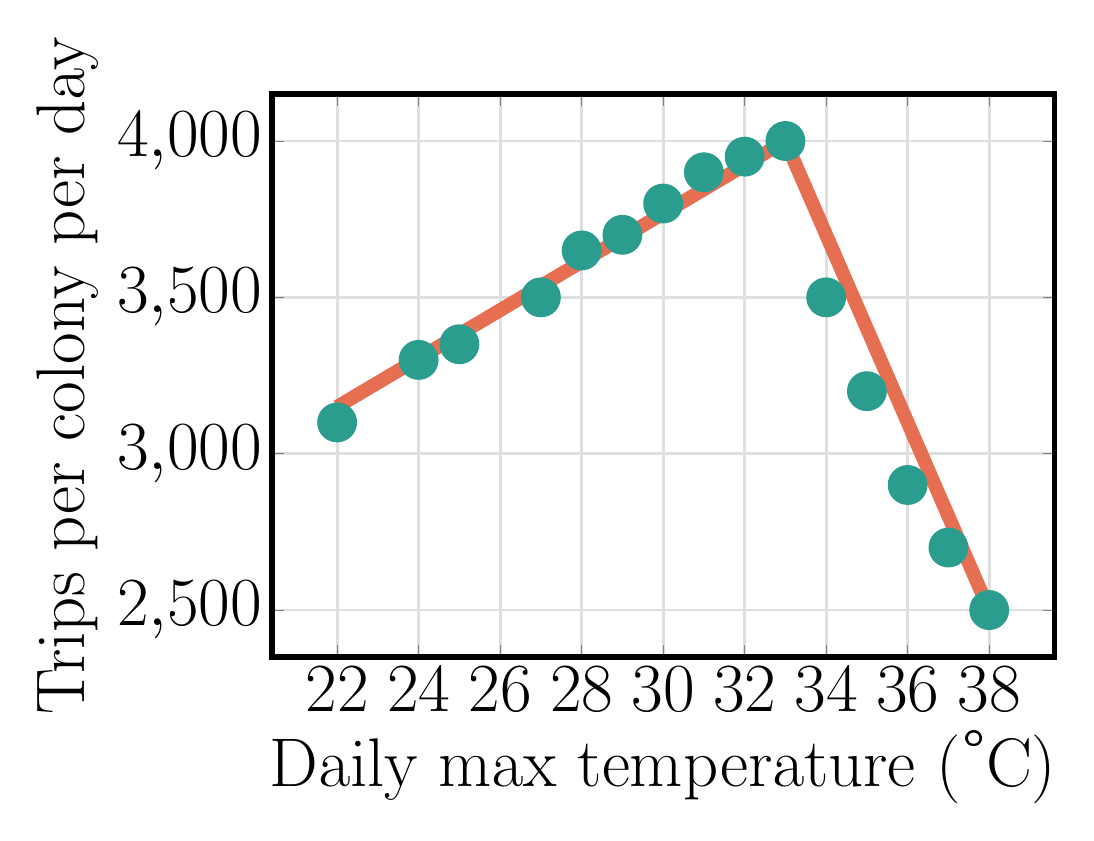
\begin{tikzpicture}
    \begin{axis}[width=0.95\linewidth, height=0.72\linewidth, font=\smallsize,
        tick label style={font=\smallsize}, xlabel={Daily max temperature (\textdegree C)},
        ylabel={Trips per colony per day}, grid=major, grid style={gray!25, line width=1pt},
        axis line style={line width=2pt}]
      \addplot[only marks, mark=*, mark size=7pt, sea] coordinates {
        (22,3100) (24,3300) (25,3350) (27,3500) (28,3650) (29,3700) (30,3800) (31,3900)
        (32,3950) (33,4000) (34,3500) (35,3200) (36,2900) (37,2700) (38,2500)};
      \addplot[line width=5pt, clay] coordinates {(22,3150) (33,4000) (38,2500)};
    \end{axis}
  \end{tikzpicture}
\end{center}
{\smallsize Each dot is a daily mean over all colonies. The line is the fitted breakpoint model.\par}

\begin{center}
  \begin{tabular}{lrr}
    \toprule
    Measure & Below 33\,\textdegree C & Above 33\,\textdegree C \\
    \midrule
    Trips per day & 3620 & 2960 \\
    Pollen (g per day) & 41.2 & 27.5 \\
    Water trips (\%) & 8 & 31 \\
    \bottomrule
  \end{tabular}
\end{center}

\keypoint{On hot days, almost a third of trips collect water for cooling instead of food.}

\columnbreak

\section{Conclusions}
\begin{enumerate}
  \item Foraging has a clear heat threshold near 33\,\textdegree C.
  \item Above it, bees trade food collection for hive cooling.
  \item Pollen income drops by a third on hot days.
\end{enumerate}

\section{Recommendations}
\begin{itemize}
  \item Provide shaded water within 50\,m of hives.
  \item Place hives where afternoon shade is available.
  \item Plan supplementary feeding after heat waves.
\end{itemize}

\section{References}
{\smallsize
\begin{enumerate}[label={[\arabic*]}]
  \item Example, R. Heat and hive thermoregulation. \emph{Journal of Example Apiculture}, 2022.
  \item Sample, T. Counting bees with sensors. \emph{Example Methods in Ecology}, 2024.
  \item Model, A. Piecewise regression for ecologists. \emph{Example Statistics Review}, 2025.
\end{enumerate}
\par}

\section{Contact}
rosa.delgado@example.edu\\
Poster presented at the Example Pollinator Symposium 2026.

\end{multicols}

\end{document}
